\section{Results}
% \begin{frame}{Results}
%     \begin{itemize}
%         \item Testing
%         \item Human Study
%     \end{itemize}
% \end{frame}

\subsection*{Technical Performance Mesurement}
\begin{frame}{Technical Performance Mesurement (TPM)}
    TPM is a set of metrics used to evaluate the performance of the system.

    \vspace*{.5cm}
    For this project evaluation, we used the following metrics:
    \begin{itemize}
        \item Classification Accuracy
        \item Latency
        \item Robustness
        \item Other Metrics
    \end{itemize}
\end{frame}

\begin{frame}{TPM \textemdash{} Classification Accuracy}
    The Classification Accuracy is the percentage of correct classifications made by the system.

    \vspace*{.5cm}
    The Confusion Matrix is a table used to describe the performance of the classification model.
\end{frame}
\begin{frame}{TMP \textemdash{} Classification Accuracy \textemdash{} Cont'd}
    Accuracy: \textbf{47.23\%}
    Confusion matrix of the validation data. 
    \begin{table}[!htbp]
        \centering
        \scalebox{.8}{
        \begin{tabular}{|c||c|c|c|c|}
            \hline
            & \textbf{Feet} & \textbf{Left Hand} & \textbf{Right Hand} & \textbf{Rest} \\
            \hline
            \hline
            \textbf{Feet} & \textbf{779} & 367 & 259 & 314 \\
            \hline
            \textbf{Left Hand} & 284 & \textbf{1005} & 189 & 258 \\
            \hline
            \textbf{Right Hand} & 356 & 243 & \textbf{840} & 268 \\
            \hline
            \textbf{Rest} & 1474 & 1188 & 1158 & \textbf{3067} \\
            \hline
        \end{tabular}
        }
    \end{table}

    Accuracy: \textbf{89.15\%}
    Confusion matrix of the GAN data. 
    \begin{table}[!htbp]
        \centering
        \scalebox{.8}{
        \begin{tabular}{|c||c|c|c|c|}
            \hline
            & \textbf{Feet} & \textbf{Left Hand} & \textbf{Right Hand} & \textbf{Rest} \\
            \hline
            \hline
            \textbf{Feet} & \textbf{824} & 104 & 38 & 34 \\
            \hline
            \textbf{Left Hand} & 16 & \textbf{961} & 1 & 22 \\
            \hline
            \textbf{Right Hand} & 28 & 51 & \textbf{789} & 132 \\
            \hline
            \textbf{Rest} & 1 & 6 & 1 & \textbf{992} \\
            \hline
        \end{tabular}
        }
    \end{table}    
\end{frame}

\begin{frame}{TPM \textemdash{} Latency}
    Latency is the time taken by the system to respond to a stimulus.
    
    Latency of the system in a real case scenario.
    \begin{figure}[!htbp]
        \scalebox{1}[1]{
        \begin{tikzpicture}
            % Horizontal line
            \draw[thick] (0,0) -- (7.6625,0);
            \draw[thick, dashed] (7.6625,0) -- (8.15,0);
            \draw[thick, -Triangle] (8.15,0) -- (10,0) node[font=\scriptsize,below left=3pt and -8pt]{\textbf{ms}};
            % \draw[thick, dashed] (9,0) -- (9.5,0);
            % \draw[thick, -Triangle] (9,0) -- (10,0) node[font=\scriptsize,below left=3pt and -8pt]{\textbf{ms}};
    
            % Start of the timeline
            \draw (0,-0.1) -- (0,0.1) node[font=\scriptsize,below left=3pt and -6pt]{\textbf{0}};
            \node[font=\scriptsize,left=3pt] at (0,0) [anchor=east]{\textbf{Min}};
    
            % Image Processing Time
            \draw (0.1625, -0.1) -- (0.1625, 0.1) node[font=\scriptsize,below left=3pt and -10pt]{\textbf{\textcolor{olive}{13}}};
            \fill[purple] (0, 0.2) rectangle (0.1625, 0.4);
            
            % \draw (1, -0.1) -- (1, 0.1) node[font=\scriptsize,below left=3pt and -8pt]{\textbf{\textcolor{red}{80}}};
            % \fill[purple] (0,-0.4) rectangle (1,-0.6);
            
            % Motor Response Time
            \draw (1.4125, -0.1) -- (1.4125, 0.1) node[font=\scriptsize,below left=3pt and -10pt]{\textbf{\textcolor{olive}{113}}};
            \fill[blue] (0.1625, 0.4) rectangle (1.4125, 0.6);
    
            % \draw (2.75, -0.1) -- (2.75, 0.1) node[font=\scriptsize,below left=3pt and -10pt]{\textbf{\textcolor{red}{220}}};
            % \fill[blue] (1,-0.6) rectangle (2.75,-0.8);
    
            % Motor Response Recording Time
            \draw (7.6625, -0.1) -- (7.6625, 0.1) node[font=\scriptsize,below left=3pt and -8pt]{\textbf{\textcolor{olive}{613}}};
            \fill[red] (1.4125, 0.6) rectangle (7.6625, 0.8);
    
            % \draw (9, -0.1) -- (9, 0.1) node[font=\scriptsize,below left=3pt and -10pt]{\textbf{\textcolor{red}{720}}};
            % \fill[red] (2.75,-0.8) rectangle (9,-1);
    
            % Signal Classification Time
            \draw (8.15, -0.1) -- (8.15, 0.1) node[font=\scriptsize,below left=3pt and -10pt]{\textbf{\textcolor{olive}{615}}};
            \fill[amethyst] (7.6625, 0.8) rectangle (8.15, 1);
    
            % \draw (9.5, -0.1) -- (9.5, 0.1) node[font=\scriptsize,below left=3pt and -10pt]{\textbf{\textcolor{red}{732}}};
            % \fill[amethyst] (9,-1) rectangle (9.5,-1.2);
    
            % diff curly brace
            % \draw [decorate,decoration={brace,amplitude=5pt}] (8.15, 1) -- (9.5,1) node [anchor=south,midway,above=4pt] {\footnotesize Signal Received by Application};
        \end{tikzpicture}
        }
        \scalebox{1}[1]{
        \begin{tikzpicture}
                % Horizontal line
                \draw[thick] (0,0) -- (9,0);
                % \draw[thick, dashed] (7.6625,0) -- (8.15,0);
                % \draw[thick] (8.15,0) -- (9,0);
                \draw[thick, dashed] (9,0) -- (9.5,0);
                \draw[thick, -Triangle] (9.5,0) -- (10,0) node[font=\scriptsize,below left=3pt and -8pt]{\textbf{ms}};
    
                % Start of the timeline
                \draw (0,-0.1) -- (0,0.1) node[font=\scriptsize,below left=3pt and -6pt]{\textbf{0}};
                \node[font=\scriptsize,left=3pt] at (0,0) [anchor=east]{\textbf{Max}};
    
                % Image Processing Time
                % \draw (0.1625, -0.1) -- (0.1625, 0.1) node[font=\scriptsize,below left=3pt and -10pt]{\textbf{\textcolor{olive}{13}}};
                % \fill[purple] (0, 0.2) rectangle (0.1625, 0.4);
                
                \draw (1, -0.1) -- (1, 0.1) node[font=\scriptsize,below left=3pt and -8pt]{\textbf{\textcolor{red}{80}}};
                \fill[purple] (0,0.2) rectangle (1,0.4);
                
                % Motor Response Time
                % \draw (1.4125, -0.1) -- (1.4125, 0.1) node[font=\scriptsize,below left=3pt and -10pt]{\textbf{\textcolor{olive}{113}}};
                % \fill[blue] (0.1625, 0.4) rectangle (1.4125, 0.6);
    
                \draw (2.75, -0.1) -- (2.75, 0.1) node[font=\scriptsize,below left=3pt and -10pt]{\textbf{\textcolor{red}{220}}};
                \fill[blue] (1,0.4) rectangle (2.75,0.6);
    
                % Motor Response Recording Time
                % \draw (7.6625, -0.1) -- (7.6625, 0.1) node[font=\scriptsize,below left=3pt and -8pt]{\textbf{\textcolor{olive}{613}}};
                % \fill[red] (1.4125, 0.6) rectangle (7.6625, 0.8);
    
                \draw (9, -0.1) -- (9, 0.1) node[font=\scriptsize,below left=3pt and -10pt]{\textbf{\textcolor{red}{720}}};
                \fill[red] (2.75,0.6) rectangle (9,0.8);
    
                % Signal Classification Time
                % \draw (8.15, -0.1) -- (8.15, 0.1) node[font=\scriptsize,below left=3pt and -10pt]{\textbf{\textcolor{olive}{614}}};
                % \fill[amethyst] (7.6625, 0.8) rectangle (8.15, 1);
    
                \draw (9.5, -0.1) -- (9.5, 0.1) node[font=\scriptsize,below left=3pt and -10pt]{\textbf{\textcolor{red}{745}}};
                \fill[amethyst] (9,0.8) rectangle (9.5,1);
    
                % diff curly brace
                % \draw [decorate,decoration={brace,amplitude=5pt}] (8.15, 1) -- (9.5,1) node [anchor=south,midway,above=4pt] {\footnotesize Signal Received by Application};    
        \end{tikzpicture}
        }
        \begin{itemize}
            \item \textcolor{purple}{Brain Processing Image Time:} 13-80 ms
            \item \textcolor{blue}{Brain Motor Response Activation Time:} 100-140 ms
            \item \textcolor{red}{BCI Motor Response Recording Time:} 500 ms
            \item \textcolor{amethyst}{Signal Classification Time:} 1.10-24.67 ms
        \end{itemize}
    \end{figure}
\end{frame}
\begin{frame}{TPM \textemdash{} Robustness}
    Robustness is the ability of the system to perform well in the presence of noise or missing data.

    \begin{figure}[!htbp]
        \centering
        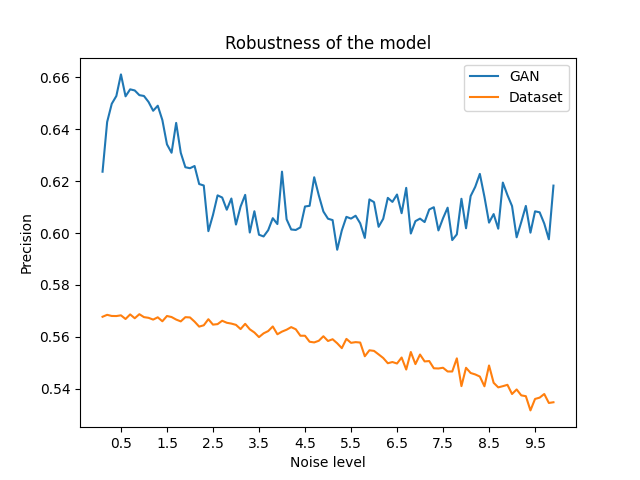
\includegraphics[width=0.8\textwidth]{figures/Testing/robustness_plot}
        % \caption{Robustness of the system in case of noise in the data.}\label{fig:robustness}
    \end{figure}
\end{frame}
\begin{frame}{TPM \textemdash{} Other Metrics}
    \begin{itemize}
        \item \textbf{Portability}: Written in Python with Torch for CUDA
        \item \textbf{Efficiency}: Can run on most modern Hardware Platforms
        \item \textbf{Maintainability}: 6.55 PyLint Score
        \item \textbf{System Resource Usage}
    \end{itemize}
    \vspace*{-.5cm}
    \begin{table}[!htbp]
        \centering
        \scalebox{.8}{
        \begin{tabular}{|c||c|c|c|}
            \hline
            \textbf{Resource} & \textbf{Minimum Usage} & \textbf{Average Usage} & \textbf{Maximum Usage} \\
            \hline
            \hline
            K-FLOPS & 754 & 754 & 754\\
            \hline
            CPU Memory & 30 KB & 47 KB & 90 KB \\
            \hline
            GPU CUDA Memory & 277 KB & 17.7 MB  & 41.3 MB \\
            \hline
        \end{tabular}
        }
        % \caption{Efficiency of the system in terms of resource usage.}
    \end{table}
\end{frame}


\subsection*{Human Study}
\begin{frame}{Human Study}
    The Human Study is a set of experiments conducted on human subjects to evaluate the system's performance.

    It is used to:
    \begin{itemize}
        \item Identify System Issues
        \item Identify Improvement Areas
        \item Evaluate User Experience
        \item Validate the System
    \end{itemize}
\end{frame}
\begin{frame}{Human Study \textemdash{} Study Design}
    \begin{figure}
        \centering
        \begin{tikzpicture}[
            squarednode/.style={rectangle, draw=black, very thick, minimum size=5mm},
            ]
            \node[] (none) {~};
            \node[] (none2) [below=of none] {~};
            \node[squarednode] (controlled) [right=of none] {Setup Controlled Environment};
            \node[squarednode] (select) [below=of controlled] {Select Participants};
            \node[] (none3) [below=of select] {~};
            \node[squarednode] (game) [below=of none2] {Play Video Game};
            \node[squarednode, dashed] (data_collection) [right=of game] {Data Collection};
            \node[squarednode] (survey) [below=of none3] {User Experience Survey};
            \node[squarednode] (improve) [below=of survey] {Improve System};

            \draw[->] (controlled) -- (select);
            \draw[->] (select) -- (game);
            \draw[->] (game) -- (survey);
            \draw[->, dashed] (survey) -- (improve);
            \draw[->, dashed] (game) -- (data_collection);
            \draw[->, dashed] (data_collection) to[out=0, in=0] (improve);
        \end{tikzpicture}
    \end{figure}
\end{frame}
\begin{frame}{Human Study \textemdash{} Participants Selection}
    % \begin{itemize}
    %     \item Informed Volunteers
    %     \item Healthy Adults
    %     \item No History of Neurological Disorders
    % \end{itemize}
    % To Sentences:
    The study will be conducted on informed healthy adult volunteers with no history of neurological disorders.

    To allow:
    \begin{itemize}
        \item Accurate Data Collection
        \item Reliable Results
        \item Ethical Conduct
        \item Safety of Participants
    \end{itemize}
\end{frame}
% \begin{frame}{Human Study \textemdash{} Procedure}
%     \begin{itemize}
%         \item Play Game for Predetermined Time
%         \item Fill Out User Experience Survey
%         \item Single Session
%         \item Flexible Environment 
%     \end{itemize}
% \end{frame}
% \begin{frame}{Human Study \textemdash{} Game Design}
%     \begin{itemize}
%         \item Engaging Game
%         \item Simple Controls
%     \end{itemize}
% \end{frame}
\begin{frame}{Human Study \textemdash{} Data Collection}
    % \begin{itemize}
    %     \item Screen Recording with Microphone
    %     \item Multiple Data Collection Points
    %     \item Identify System Issues
    %     \item Identify Improvement Areas
    % \end{itemize}
    % To Sentences:
    The Data Collection is a fundamental step to identify system issues and improvement areas.

    It will be done through screen recording with microphone and multiple data collection points.

    The data will be used to:
    \begin{itemize}
        \item Verify System Usability
        \item Verify User Experience
        \item Verify User Acceptance
        \item Validate the System
        \item Search Points of Failure
        \item Improve the System preformances and accuracy
    \end{itemize}
\end{frame}
\begin{frame}{Human Study \textemdash{} User Experience Survey}
    % \begin{itemize}
    %     \item Likert Scale (from 1 to 10)
    %     \item System Usability Scale (SUS)
    %     \item Game Experience Questionnaire
    %     \item Concise and Easy to Understand
    % \end{itemize}
    % To Sentences:
    The User Experience Survey is a set of questions to evaluate the system's usability and user experience.

    \vspace{.5cm}
    In this study, the survey will include a set of questions scored using the Likert Scale (from 1 to 10), including questions from the System Usability Scale (SUS) and the Game Experience Questionnaire.

    \vspace*{.5cm}
    The survey will be concise and easy to understand.
\end{frame}
\subsection*{Pre-testing}
\begin{frame}{Pre-Testing}
    % \begin{itemize}
    %     \item Verify the System Usability
    %     \item Verify Real-Time Data Collection
    %     \item Verify Lag and Delays
    %     \item Search Points of Failure
    % \end{itemize}
    % To Sentences:
    The Pre-Testing is a set of experiments conducted before the Human Study to verify the system's usability and real-time data collection.

    \vspace*{.5cm}
    In this study, we completed the pre-testing phase and identified Robustness as a critical point of failure, therefore we could not proceed with the Human Study.

    \vspace*{.5cm}
    The data collected will be used to improve the system's performance and accuracy.
\end{frame}
\begin{frame}{Pre-Testing \textemdash{} Headset}
    \begin{figure}
        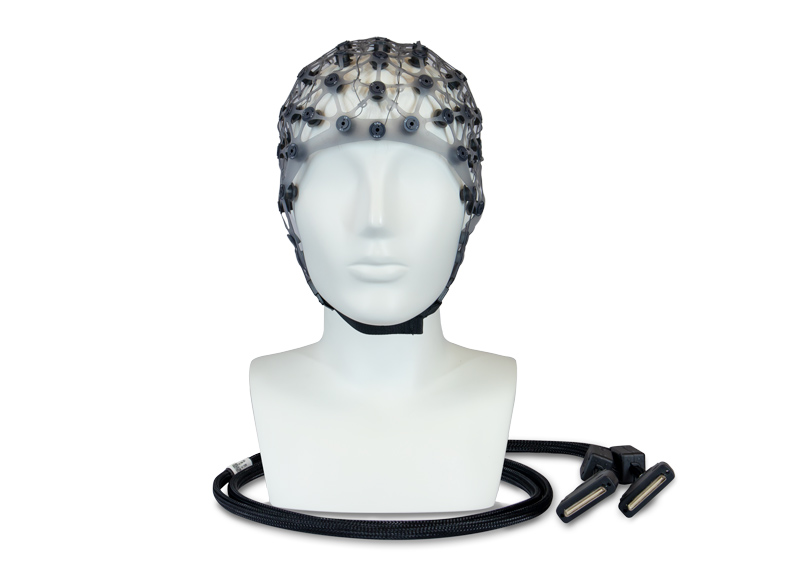
\includegraphics[width=\textwidth]{figures/results/EEG_CAP}
    \end{figure}
\end{frame}
\begin{frame}{Pre-Testing \textemdash{} EEG Cap Layout}
    \begin{figure}
        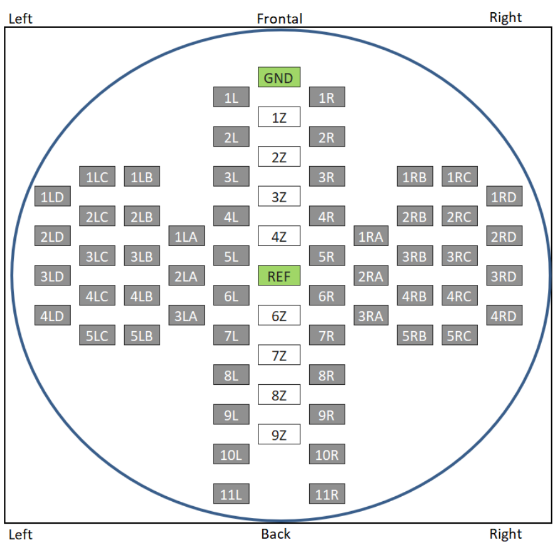
\includegraphics[width=.65\textwidth]{figures/results/CAP_Layout}
    \end{figure}
\end{frame}

% \subsection*{Technical Performance Mesurement}
\begin{frame}{Technical Performance Mesurement}
    \begin{itemize}
        \item Classification Accuracy
        \item Latency
        \item Robustness
        \item Other Metrics
    \end{itemize}
\end{frame}

\begin{frame}{TPM \textemdash{} Classification Accuracy}

\begin{table}[!htbp]
    \centering
    \begin{tabular}{|c||c|c|c|c|}
        \hline
        & \textbf{Feet} & \textbf{Left Hand} & \textbf{Right Hand} & \textbf{Rest} \\
        \hline
        \hline
        \textbf{Feet} & \textbf{779} & 367 & 259 & 314 \\
        \hline
        \textbf{Left Hand} & 284 & \textbf{1005} & 189 & 258 \\
        \hline
        \textbf{Right Hand} & 356 & 243 & \textbf{840} & 268 \\
        \hline
        \textbf{Rest} & 1474 & 1188 & 1158 & \textbf{3067} \\
        \hline
    \end{tabular}
    \caption{Confusion matrix of the validation dataset. \textbf{47.23\%} Accuracy}
\end{table}
\begin{table}[!htbp]
    \centering
    \begin{tabular}{|c||c|c|c|c|}
        \hline
        & \textbf{Feet} & \textbf{Left Hand} & \textbf{Right Hand} & \textbf{Rest} \\
        \hline
        \hline
        \textbf{Feet} & \textbf{824} & 104 & 38 & 34 \\
        \hline
        \textbf{Left Hand} & 16 & \textbf{961} & 1 & 22 \\
        \hline
        \textbf{Right Hand} & 28 & 51 & \textbf{789} & 132 \\
        \hline
        \textbf{Rest} & 1 & 6 & 1 & \textbf{992} \\
        \hline
    \end{tabular}
    \caption{Confusion matrix of the GAN data. \textbf{89.15\%} Accuracy}
\end{table}

\end{frame}
\begin{frame}{TPM \textemdash{} Latency}
    \begin{figure}[!htbp]
        \scalebox{1}[1]{
        \begin{tikzpicture}
            % Horizontal line
            \draw[thick] (0,0) -- (7.6625,0);
            \draw[thick, dashed] (7.6625,0) -- (8.15,0);
            \draw[thick, -Triangle] (8.15,0) -- (10,0) node[font=\scriptsize,below left=3pt and -8pt]{\textbf{ms}};
            % \draw[thick, dashed] (9,0) -- (9.5,0);
            % \draw[thick, -Triangle] (9,0) -- (10,0) node[font=\scriptsize,below left=3pt and -8pt]{\textbf{ms}};
    
            % Start of the timeline
            \draw (0,-0.1) -- (0,0.1) node[font=\scriptsize,below left=3pt and -6pt]{\textbf{0}};
            \node[font=\scriptsize,left=3pt] at (0,0) [anchor=east]{\textbf{Min}};
    
            % Image Processing Time
            \draw (0.1625, -0.1) -- (0.1625, 0.1) node[font=\scriptsize,below left=3pt and -10pt]{\textbf{\textcolor{olive}{13}}};
            \fill[purple] (0, 0.2) rectangle (0.1625, 0.4);
            
            % \draw (1, -0.1) -- (1, 0.1) node[font=\scriptsize,below left=3pt and -8pt]{\textbf{\textcolor{red}{80}}};
            % \fill[purple] (0,-0.4) rectangle (1,-0.6);
            
            % Motor Response Time
            \draw (1.4125, -0.1) -- (1.4125, 0.1) node[font=\scriptsize,below left=3pt and -10pt]{\textbf{\textcolor{olive}{113}}};
            \fill[blue] (0.1625, 0.4) rectangle (1.4125, 0.6);
    
            % \draw (2.75, -0.1) -- (2.75, 0.1) node[font=\scriptsize,below left=3pt and -10pt]{\textbf{\textcolor{red}{220}}};
            % \fill[blue] (1,-0.6) rectangle (2.75,-0.8);
    
            % Motor Response Recording Time
            \draw (7.6625, -0.1) -- (7.6625, 0.1) node[font=\scriptsize,below left=3pt and -8pt]{\textbf{\textcolor{olive}{613}}};
            \fill[red] (1.4125, 0.6) rectangle (7.6625, 0.8);
    
            % \draw (9, -0.1) -- (9, 0.1) node[font=\scriptsize,below left=3pt and -10pt]{\textbf{\textcolor{red}{720}}};
            % \fill[red] (2.75,-0.8) rectangle (9,-1);
    
            % Signal Classification Time
            \draw (8.15, -0.1) -- (8.15, 0.1) node[font=\scriptsize,below left=3pt and -10pt]{\textbf{\textcolor{olive}{615}}};
            \fill[amethyst] (7.6625, 0.8) rectangle (8.15, 1);
    
            % \draw (9.5, -0.1) -- (9.5, 0.1) node[font=\scriptsize,below left=3pt and -10pt]{\textbf{\textcolor{red}{732}}};
            % \fill[amethyst] (9,-1) rectangle (9.5,-1.2);
    
            % diff curly brace
            % \draw [decorate,decoration={brace,amplitude=5pt}] (8.15, 1) -- (9.5,1) node [anchor=south,midway,above=4pt] {\footnotesize Signal Received by Application};
        \end{tikzpicture}
        }
        \scalebox{1}[1]{
        \begin{tikzpicture}
                % Horizontal line
                \draw[thick] (0,0) -- (9,0);
                % \draw[thick, dashed] (7.6625,0) -- (8.15,0);
                % \draw[thick] (8.15,0) -- (9,0);
                \draw[thick, dashed] (9,0) -- (9.5,0);
                \draw[thick, -Triangle] (9.5,0) -- (10,0) node[font=\scriptsize,below left=3pt and -8pt]{\textbf{ms}};
    
                % Start of the timeline
                \draw (0,-0.1) -- (0,0.1) node[font=\scriptsize,below left=3pt and -6pt]{\textbf{0}};
                \node[font=\scriptsize,left=3pt] at (0,0) [anchor=east]{\textbf{Max}};
    
                % Image Processing Time
                % \draw (0.1625, -0.1) -- (0.1625, 0.1) node[font=\scriptsize,below left=3pt and -10pt]{\textbf{\textcolor{olive}{13}}};
                % \fill[purple] (0, 0.2) rectangle (0.1625, 0.4);
                
                \draw (1, -0.1) -- (1, 0.1) node[font=\scriptsize,below left=3pt and -8pt]{\textbf{\textcolor{red}{80}}};
                \fill[purple] (0,0.2) rectangle (1,0.4);
                
                % Motor Response Time
                % \draw (1.4125, -0.1) -- (1.4125, 0.1) node[font=\scriptsize,below left=3pt and -10pt]{\textbf{\textcolor{olive}{113}}};
                % \fill[blue] (0.1625, 0.4) rectangle (1.4125, 0.6);
    
                \draw (2.75, -0.1) -- (2.75, 0.1) node[font=\scriptsize,below left=3pt and -10pt]{\textbf{\textcolor{red}{220}}};
                \fill[blue] (1,0.4) rectangle (2.75,0.6);
    
                % Motor Response Recording Time
                % \draw (7.6625, -0.1) -- (7.6625, 0.1) node[font=\scriptsize,below left=3pt and -8pt]{\textbf{\textcolor{olive}{613}}};
                % \fill[red] (1.4125, 0.6) rectangle (7.6625, 0.8);
    
                \draw (9, -0.1) -- (9, 0.1) node[font=\scriptsize,below left=3pt and -10pt]{\textbf{\textcolor{red}{720}}};
                \fill[red] (2.75,0.6) rectangle (9,0.8);
    
                % Signal Classification Time
                % \draw (8.15, -0.1) -- (8.15, 0.1) node[font=\scriptsize,below left=3pt and -10pt]{\textbf{\textcolor{olive}{614}}};
                % \fill[amethyst] (7.6625, 0.8) rectangle (8.15, 1);
    
                \draw (9.5, -0.1) -- (9.5, 0.1) node[font=\scriptsize,below left=3pt and -10pt]{\textbf{\textcolor{red}{745}}};
                \fill[amethyst] (9,0.8) rectangle (9.5,1);
    
                % diff curly brace
                % \draw [decorate,decoration={brace,amplitude=5pt}] (8.15, 1) -- (9.5,1) node [anchor=south,midway,above=4pt] {\footnotesize Signal Received by Application};    
        \end{tikzpicture}
        }
        \begin{itemize}
            \item \textcolor{purple}{Brain Processing Image Time:} 13-80 ms
            \item \textcolor{blue}{Brain Motor Response Activation Time:} 100-140 ms
            \item \textcolor{red}{BCI Motor Response Recording Time:} 500 ms
            \item \textcolor{amethyst}{Signal Classification Time:} 1.10-24.67 ms
        \end{itemize}
        \caption{Latency of the system in a real case scenario.}\label{fig:latency}
    \end{figure}
\end{frame}
\begin{frame}{TPM \textemdash{} Robustness}
    \begin{figure}[!htbp]
        \centering
        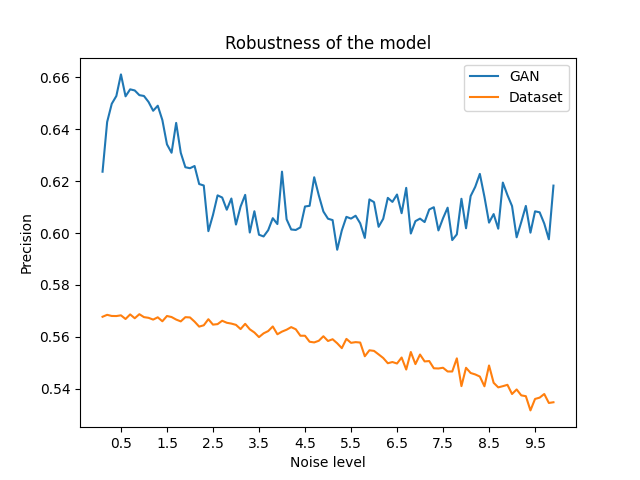
\includegraphics[width=0.8\textwidth]{figures/Testing/robustness_plot}
        \caption{Robustness of the system in case of noise in the data.}\label{fig:robustness}
    \end{figure}
\end{frame}
\begin{frame}{TPM \textemdash{} Other Metrics}
    \begin{itemize}
        \item Portability: Written in Python with Torch for CUDA
        \item Efficiency: Can run on most modern Hardware Platforms
        \item Maintainability: 6.55 PyLint Score
    \end{itemize}
    \begin{table}[!htbp]
        \centering
        \scalebox{.8}{
        \begin{tabular}{|c||c|c|c|}
            \hline
            \textbf{Resource} & \textbf{Minimum Usage} & \textbf{Average Usage} & \textbf{Maximum Usage} \\
            \hline
            \hline
            K-FLOPS & 754 & 754 & 754\\
            \hline
            CPU Memory & 30 KB & 47 KB & 90 KB \\
            \hline
            GPU CUDA Memory & 277 KB & 17.7 MB  & 41.3 MB \\
            \hline
        \end{tabular}
        }
        \caption{Efficiency of the system in terms of resource usage.}
    \end{table}
\end{frame}

% \subsection*{Human Study}
\begin{frame}{Human Study}
    \begin{itemize}
        \item Study Design
        \item Participants
        \item Procedure
        \item Game Design
        \item Data Collection
        \item User Experience Survey
        \item Pre-Testing
    \end{itemize}
\end{frame}
\begin{frame}{Human Study \textemdash{} Study Design}
    \begin{itemize}
        \item Play Video Game with EEG Headset and Motor Imagery
        \item Controlled Environment
        \item User Experience Survey
    \end{itemize}
\end{frame}
\begin{frame}{Human Study \textemdash{} Participants}
    \begin{itemize}
        \item Healthy Adults
        \item No History of Neurological Disorders
        \item Informed Participation
    \end{itemize}
\end{frame}
\begin{frame}{Human Study \textemdash{} Procedure}
    \begin{itemize}
        \item Play Game for Predetermined Time
        \item Fill Out User Experience Survey
        \item Single Session
        \item Flexible Environment 
    \end{itemize}
\end{frame}
\begin{frame}{Human Study \textemdash{} Game Design}
    \begin{itemize}
        \item Engaging Game
        \item Simple Controls
    \end{itemize}
\end{frame}
\begin{frame}{Human Study \textemdash{} Data Collection}
    \begin{itemize}
        \item Screen Recording with Microphone
        \item Multiple Data Collection Points
        \item Identify System Issues
        \item Identify Improvement Areas
    \end{itemize}
\end{frame}
\begin{frame}{Human Study \textemdash{} User Experience Survey}
    \begin{itemize}
        \item Likert Scale (from 1 to 10)
        \item Included System Usability Scale (SUS)
        \item Included Game Experience Questionnaire
        \item Concise and Easy to Understand
    \end{itemize}
\end{frame}
\begin{frame}{Human Study \textemdash{} Pre-Testing}
    \begin{itemize}
        \item Verify the System Usability
        \item Verify Real-Time Data Collection
        \item Verify Lag and Delays
        \item Search Points of Failure
        \item Identified need for Fine Tuning
    \end{itemize}
\end{frame}

